\documentclass[11pt,letterpaper]{article}
\usepackage[margin=1in]{geometry}
\usepackage{graphicx}
\usepackage[font=footnotesize,labelfont=bf,width=5in]{caption}
\usepackage{amsmath}

\renewcommand{\baselinestretch}{1.3}

\title{{Automatic Least-Effort Contextual Learning}}
\author{Lucas E. Morales\\{\tt \{lucasem\}}
\and Kevin Ellis\\{\tt \{ellisk\}}
\and Joshua Tenenbaum\\{\tt \{jbt\}}}
\date{}


\begin{document}

\maketitle

\begin{abstract}
  In the field of artificial intelligence, most learning mechanisms are
  either inherently specialized or have a flat knowledge base that makes
  them only useful when confined to a single domain, reducing the capability
  of both handling complex problems and specializing in multiple domains.
  This project is to design a contextual knowledge system called Scale-free
  Knowledge Network (SKN). We augment learning mechanisms to utilize this
  knowledge system in a manner that reduces the intractability of hard
  problems by leveraging compositionality rooted in implicit relationships
  between learned knowledge artifacts.
\end{abstract}


\section{Introduction}

Knowledge, as a familiarity with things, is attained by experience via
learning. Learning mechanisms both construct and consume knowledge, allowing
for higher order learning compared to the base of sensory input. This
interaction must not be immediately free to use all knowledge: a particular
context must motivate certain knowledge artifacts to be readily available
while setting others further apart, depending on their relationships to
those in contextual proximity.

To contextualize knowledge in an abstract manner, we develop the SKN
framework ({\bf S}cale-free {\bf K}nowledge {\bf N}etwork). Knowledge is
represented as distinct items of information and their relations in the
structure of a connected network. The network is constructed by preferential
``least effort'' attachment \cite{barabasi99}\cite{cancho03}, where a new
knowledge artifact joins the network with relations to the contextual
knowledge from which it was learned. This network is scale-free --- it
conforms to a mathematical pattern similar to that of Zipf's Law and Pareto
distributions \cite{zipf49}\cite{barabasi16}, where the degree of
connectivity for nodes in the network follow a class of power law
distributions. The resulting system provides automatic compositionality for
learning mechanisms which rely on knowledge artifacts, enabling rapid
learning of rich models \cite{lake16}.


\section{Relevant Works}

In the discipline of artificial intelligence, much effort is placed on
designing accurate learning mechanisms. These learning mechanisms are
either designed for a particular domain, or designed to specialize
given consistent domain-specific input. Special-purpose learning mechanisms
include visual object recognition systems based on the human visual cortex
\cite{serre07}, handwritten character identification and generation
\cite{lake15}, visual feature modification of images \cite{kulkarni15}, and
sound texture perception and synthesis \cite{mcdermott11}. General-purpose
learning mechanisms include hierarchical Bayesian methods
\cite{tenenbaum01}, program learning \cite{liang10}\cite{dechter13},
inductive logic programming \cite{lavrac94}\cite{muggleton15}, and
generative adversarial networks \cite{goodfellow14}.

Each of these mechanisms are remarkable, but lack the generality that is
apparent in human cognition. Even the general-purpose mechanisms, while
capable of being applied to many domains, are only practical when restricted
to a single domain, as a specialized instantiation of the mechanism. The
need for specialization makes general-purpose mechanisms unappealing in
practice, because a special-purpose mechanism could outperform it. This
stems, in part, from a problem of \emph{knowledge}, for which learning
mechanisms have some internal representation. Those representations are
mechanism-specific, and are generally used without hierarchy. Making all
knowledge flat in this manner yields systems that are only performant when
confined to a single domain and flawed as a model of cognition due to the
reduced capability of both handling very complex problems and specializing
in multiple domains.

Theories for cognitive architecture have pursued solving these problems.
ACT* \cite{anderson83} is a system which utilizes memory according to a
degree of activation, where activation spreads to favor information most
related to the immediate context. ACT* relates items of memory with a matrix
pairing the strength of connection between any two items, which restricts
memory capacity with a flat representation of knowledge and is therefore
lacking in the same vein as the mechanisms mentioned above. Soar
\cite{newell94} is another system of cognitive architecture which traverses
memory by recognition as pattern-matching on production rules. Soar has
unstructured sets of memory and relies on ``chunking'' to convert
problem-solving into memory, where chunking is essentially a form of
learning by generation of production rules with implicit generalization
about the context it informs. Soar doesn't have implicit relationships
between items of knowledge like ACT*, and has limited explicit relationships
about context as a hierarchical tuple of subgoals, problem spaces, states,
and operators (hierarchical in that if an item of the tuple is specified,
all subsequent items are nullable). Soar relies on efficient chunking to
reduce the complexity of problem solving.

Preferential ``least-effort'' attachment and resulting power-law
distributions have been reported heavily over the last century, from urn
models and Yule processes describing the statistics of the evolution of
simple mathematical systems, to Zipf's Law describing patterns in social
wealth and natural language, to the Matthew effect describing analogous
patterns in psychosocial processes, to the emergence of scale-free networks
and its presence in protein interactions, linguistics, citations, and many
other systems \cite{yule25}\cite{zipf49}\cite{merton68}\cite{barabasi99}%
\cite{jeong01}\cite{cancho01}\cite{price02}.
We model non-flat sets of knowledge artifacts using a scale-free network
based on intuitive traits of cognition: 
\begin{itemize}
  \item \emph{Growth}, the learning and discovery of new knowledge artifacts
    expanding and/or modifying a knowledge-base.
  \item \emph{Least-effort attachment}, the construction of relations
    between a new knowledge artifact and its antecedents. These relations
    are not random, but instead associate according to relevance.
\end{itemize}
Presence of these two traits in systems have been shown effective in
yielding scale-free networks. While the flat representations described
earlier in this section yields an average distance of $\langle d\rangle=1$
(corresponding to the immediate access to every item in the network and an
obvious scale to the network), scale-free networks yield an average distance
of $\langle d\rangle\sim\lg\lg N$ for network size $N$. Even with massive
network sizes it's still easy to travel from one point of the network to
another. The lack of scale to the network refers to the variety of
generally-useful (high degree) and highly-specialized (low degree) items
within the same network, a feature which inherently encodes a metric of
utility in the network structure.

The goal of SKN is to augment learning mechanisms around \emph{contextual}
knowledge in a manner that reduces the intractability of hard problems by
implicitly relating knowledge in a non-flat structure, enabling
compositionality at arbitrary scale. In terms of the Marr-Poggio levels of
analysis \cite{marr78}, SKN serves as a tool on the algorithmic level of
abstraction, not as a description of hardware-level structure --- analogous
to the World Wide Web operating at a higher level over the Internet.


\section{Technical Approach}

\begin{figure}[h]
\centering
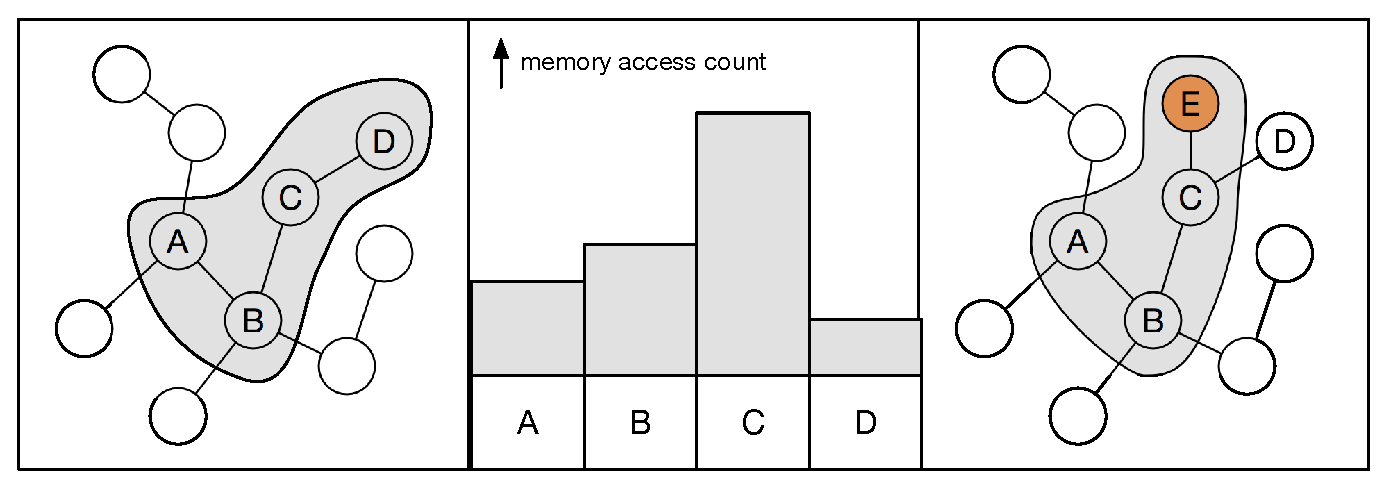
\includegraphics[scale=.5]{sf_add.eps}
\caption{The first pane shows a knowledge network, and a shaded region
  representing the active context. The second pane shows the memory accesses
  to particular knowledge artifacts leading up to the addition of a new
  knowledge artifact. The third pane shows the new knowledge network, with
  the additional knowledge artifact.}
\label{fig:sf_add}
\end{figure}

\begin{table}[h]
  \begin{center}
  \begin{tabular}{|l|p{4in}|}
    \hline
    {\tt Get() \{Item\}}     & Yields the set of items in the active context \\
                               \hline
    {\tt Explore() \{Item\}} & Yields the set of items within one edge of
                               the active context \\ \hline
    {\tt Orient(ID)}         & Shifts context to focus on the item identified
                               by the given ID \\ \hline
    {\tt Add(Item)}          & Adds an item to the knowledge network \\ \hline
  \end{tabular}
  \end{center}
\caption{Methods on an instance of the knowledge network.}
\label{tab:sf_get}
\end{table}


The SKN system implements a knowledge abstraction, on par with typical
non-hierarchical sets or addressed memory. We refer to a small motivated
subnet of the knowledge network as the {\em context}. We provide a simple
interface for interacting with knowledge where all interactions either
retrieve information related to the current context or adjust the context
within the knowledge network, outlined in Table \ref{tab:sf_get}, where {\tt
Item} is a structure containing a unique identifier, a symbolic tag denoting
which mechanism can understand the item's content, and the arbitrary content
itself. Only the {\tt Add} and {\tt Orient} methods have the potential to
augment the active context. The context itself is sized according to the
maximum degree of a node in a scale-free network, based on network size $N$
and degree exponent $\gamma$ satisfying $2<\gamma<3$:
\[k_{\text{max}} \sim N^{\frac1{\gamma-1}}\]
The {\tt Add} method automatically adds a new item of
knowledge to the network, and adjusts the context to include the new item,
illustrated in Figure \ref{fig:sf_add}.

The automatic attachment follows a least-effort procedure where the new
node's connections are determined using a popular-based probabilistic subset
selection technique equivalent to a non-initial iteration of the Indian
Buffet Process (IBP) with parameter $\alpha=0$ \cite{griffiths11}. For every
node $\mathcal{I}_j\in\{\mathcal{I}_i\}_{i=1}^k$ in the context we have
$m_j$, a count of accesses to $\mathcal{I}_j$ since the last context-switch.
Additionally, we define $M=\sum_{i=1}^km_i$ as the total count of knowledge
artifact accesses since the last context-switch. The new node attaches to
node $\mathcal{I}_j$ according to Bernoulli$\left(\frac{m_j}{M}\right)$.
% IBP doesn't guarantee non-empty set:
If no connections are made for the new node, a single connection is forced
using an iteration of the Chinese Restaurant Process (CRP) with parameter
$\alpha=0$ and an initial configuration of $k$ tables associated with nodes
in the context where the occupancy of each table is the count of memory
accesses to its corresponding node. This yields the same probability of
selecting a node as the IBP, but guarantees exactly one connection.

While this attachment procedure follows a least-effort scheme, emergent
properties of the network (such as the degree exponent $\gamma$) are
ultimitely determined by how a learning mechanism interacts with knowledge,
and no theoretical guarantee of the scale-free property can be made. A
guarantee of the scale-free property can come from attachments being made to
nodes according to their degree of connectivity (rather than memory
accesses). This is not anticipated to be problematic for learning mechanisms
which interact with knowledge artifacts according to their utility, because
the tasks that a mechanism faces tend to utilize certain concepts more than
others, naturally resulting in memory accesses that are proportional to
their high utility and thus correlated with high degree of connectivity in
the network.

\section{Experiments}

To experiment with SKN, consider the class of problems for which this system
would excel: complex domains where modular knowledge improves the efficiency
of completing relevant tasks. There are many learning mechanisms which are
suitable for experimentation, such as inductive logic programming (ILP)
systems or algorithms which perform search on a grammar. Distinct knowledge
artifacts for ILP systems could be sets of predicates, and for grammar
search systems they could be language artifacts which construct a mixture
model on which search is performed.

We augment an algorithm which performs search on a learned expressive
grammar, the EC algorithm \cite{dechter13}. The augmentation will define the
grammar based on learned language artifacts stored in the context, rather
than artifacts stored in a small bounded set. The augmented EC algorithm
will be tested in the domain of string transformation, chosen because it has
potential for common underlying structure between tasks. Results will be
compared to the original EC algorithm.

This section is very much {\bf TODO}.


\section{Conclusion}

We introduce SKN, a knowledge abstraction to improve learning mechanisms by
utilizing context in a scale-free network, with the purpose of better
modeling memory and knowledge in a convenient paradigm that fits both the
intuitive architecture of cognition and the programmatic methods of
computation that govern technology.


\section{Future Work}

The SKN system can be utilized in many different ways. By connecting many
learning mechanisms to the same knowledge network, interoperability between
distinct learning mechanisms such as for vision and sound can result in
proximal --- and perhaps even shared --- knowledge artifacts representing
the same symbol being percieved by different mechanisms. Because learning
mechanisms treat knowledge artifacts as first-class objects that can be
observed, modified, or created, the mechanisms don't necessarily have to be
restricted to \emph{learners} --- the introduction of \emph{actors} as
mechanisms would yield a powerful production system conditioned on
contextual knowledge and immediate circumstance. Supplemented with support
for direct communication between mechanisms, the mechanisms would be more
fittingly referred to as
\emph{agents} \cite{minsky88}.


\begin{thebibliography}{}
  \bibitem{barabasi99}
    Barab\'asi, A. L., \& Albert, R. (1999).
    Emergence of scaling in random networks.
    \emph{Science}, 286(5439), 509-512.
  \bibitem{cancho03} i Cancho, R. F., \& Solé, R. V. (2003)
    Least effort and the origins of scaling in human language.
    In \emph{Proceedings of the National Academy of Sciences} 100(3), 788-791.
  \bibitem{zipf49} Zipf, G. K. (1949).
    Human Behaviour and the Principle of Least-Effort.
  \bibitem{barabasi16}
    Barab\'asi, A. L. (2016).
    \emph{Network science}.
    Cambridge University Press.
  \bibitem{lake16} Lake, B. M., Ullman, T. D., Tenenbaum, J. B., \& Gershman, S. J. (2016).
    Building machines that learn and think like people.
    \emph{arXiv preprint arXiv:1604.00289}.
%  \bibitem{clauset09} Clauset A., Shalizi, C. R., \& Newman M. E. J.  (2009)
%    Power-law distributions in empirical data.
%    \emph{SIAM Review} 51(4), 661-703 (arXiv:0706.1062, doi:10.1137/070710111)
  \bibitem{serre07}
    Serre, T., Oliva, A., \& Poggio, T. (2007).
    A feedforward architecture accounts for rapid categorization.
    In \emph{Proceedings of the National Academy of Sciences}, 104(15), 6424-6429.
  \bibitem{lake15} Lake, B. M., Salakhutdinov, R., \& Tenenbaum, J. B. (2015).
    Human-level concept learning through probabilistic program induction.
    \emph{Science}, 350(6266), 1332-1338.
  \bibitem{kulkarni15}
    Kulkarni, T. D., Whitney, W. F., Kohli, P., \& Tenenbaum, J. (2015).
    Deep convolutional inverse graphics network.
    In \emph{Advances in Neural Information Processing Systems} (pp. 2539-2547).
  \bibitem{mcdermott11}
    McDermott, J. H., \& Simoncelli, E. P. (2011).
    Sound texture perception via statistics of the auditory periphery:
    evidence from sound synthesis.
    \emph{Neuron}, 71(5), 926-940.
  \bibitem{tenenbaum01}
    Tenenbaum, J. B., \& Griffiths, T. L. (2001).
    The rational basis of representativeness.
    In \emph{Proceedings of the 23rd annual conference of the Cognitive
    Science Society} (p. 103641).
  \bibitem{liang10}
    Liang, P., Jordan, M. I., \& Klein, D. (2010).
    Learning programs: a hierarchical Bayesian approach.
    \emph{International Conference on Machine Learning}: 639–646
  \bibitem{dechter13}
    Dechter, E., Malmaud, J., Adams, R. P., \& Tenenbaum, J. B. (2013).
    Bootstrap Learning via Modular Concept Discovery.
    In \emph{IJCAI}.
  \bibitem{lavrac94}
    Lavrac, N., \& Dzeroski, S. (1994).
    Inductive Logic Programming.
    In \emph{WLP} (pp. 146-160).
  \bibitem{muggleton15}
    Muggleton, S. H., Lin, D., \& Tamaddoni-Nezhad, A. (2015).
    Meta-interpretive learning of higher-order dyadic datalog: Predicate
    invention revisited.
    \emph{Machine Learning, 100}(1), 49-73.
  \bibitem{goodfellow14}
    Goodfellow, I., Pouget-Abadie, J., Mirza, M., Xu, B., Warde-Farley, D.,
    Ozair, S., ... \& Bengio, Y. (2014).
    Generative adversarial nets.
    In \emph{Advances in Neural Information Processing Systems} (pp.
    2672-2680).
  \bibitem{anderson83}
    Anderson, J. R. (1983).
    \emph{The architecture of cognition}. Psychology Press.
  \bibitem{newell94}
    Newell, A. (1994).
    \emph{Unified theories of cognition}. Harvard University Press.
  \bibitem{yule25}
    Udny Yule, G. (1925).
    A mathematical theory of evolution, based on the conclusions of Dr. JC Willis, FRS.
    \emph{Philosophical Transactions of the Royal Society of London Series B}, 213, 21-87.
  \bibitem{merton68}
    Merton, R. K. (1968).
    The Matthew effect in science.
    \emph{Science, 159}(3810), 56-63.
  \bibitem{jeong01}
    Jeong, H., Mason, S. P., Barabási, A. L., \& Oltvai, Z. N. (2001).
    Lethality and centrality in protein networks.
    \emph{Nature, 411}(6833), 41-42.
  \bibitem{cancho01}
    i Cancho, R. F., \& Solé, R. V. (2001).
    The small world of human language.
    \emph{Proceedings of the Royal Society of London B: Biological Sciences, 268}(1482), 2261-2265.
  \bibitem{price02}
    de Solla Price, D. J. (2002).
    The pattern of bibliographic references indicates the nature of the scientific research front.
    \emph{Social Networks: Critical Concepts in Sociology, 4}, 328.
  \bibitem{marr78}
    Marr, D., \& Poggio, T. (1976).
    From understanding computation to understanding neural circuitry.
  \bibitem{griffiths11}
    Griffiths, T. L., \& Ghahramani, Z. (2011).
    The indian buffet process: An introduction and review.
    \emph{Journal of Machine Learning Research}, 12(Apr), 1185-1224.
%  \bibitem{hofstadter94}
%    Hofstadter, D. R., \& Mitchell, M. (1994).
%    The copycat project: A model of mental fluidity and analogy-making.
%    \emph{Advances in connectionist and neural computation theory}, 2(31-112), 29-30.
%  \bibitem{rozenberg80}
%    Rozenberg, G., \& Salomaa, A. (1980).
%    Mathematical Theory of L systems.
%    \emph{Academic Press, Inc.}.
  \bibitem{minsky88}
    Minsky, M. (1988).
    \emph{Society of mind}.
    Simon and Schuster.
\end{thebibliography}

\end{document}
